\documentclass[final]{siamltexmm}
\documentclass[10pt,a4paper]{article}

\usepackage{graphicx}
\usepackage{algorithm}
\usepackage{algorithmic}

% \usepackage[demo]{graphicx}
% \usepackage{subfig}

\newcommand{\pe}{\psi}
\def\d{\delta} 
\def\ds{\displaystyle} 
\def\e{{\epsilon}} 
\def\eb{\bar{\eta}}  
\def\enorm#1{\|#1\|_2} 
\def\Fp{F^\prime}  
\def\fishpack{{FISHPACK}} 
\def\fortran{{FORTRAN}} 
\def\gmres{{GMRES}} 
\def\gmresm{{\rm GMRES($m$)}} 
\def\Kc{{\cal K}} 
\def\norm#1{\|#1\|} 
\def\wb{{\bar w}} 
\def\zb{{\bar z}} 

% some definitions of bold math italics to make typing easier.
% They are used in the corollary.

\def\bfE{\mbox{\boldmath$E$}}
\def\bfG{\mbox{\boldmath$G$}}

\title{Deep Learning Assignment 2}
\author{Yun-shao Sung\thanks{\tt yss265@nyu.edu}
        \and Chung-Ling Yao\thanks{\tt cly264@nyu.edu}}

\begin{document}
\maketitle

\begin{abstract}
This is the report for deep learning assignment 2
\end{abstract}

\pagestyle{myheadings}
\thispagestyle{plain}

\section{More Backpropagation}
\subsection{Backpropagation through a DAG of modules}
\subsection{Batch Normalization}

\\
\section{STL-10: semi-supervised image recognition}
\subsection{Sample code}
\subsection{STL-10}


\\
\section{Visualization}
\subsection{Visualizing filters and augmentations}
\subsection{t-SNE}
Here we took all the images from val.t7b, which contains 1000 figures for total and 100 figures in each of class. To generate t-SNE embedding, we used only the first channel of each of the image, which the dimension is 1x96x96, and feed it into manifold.embedding.tsne. Then we will get the mapping result for each of the image onto the 2D space, and we can plot the figures based on the mapped coordinate.

\begin{figure}[H]
  \centering
    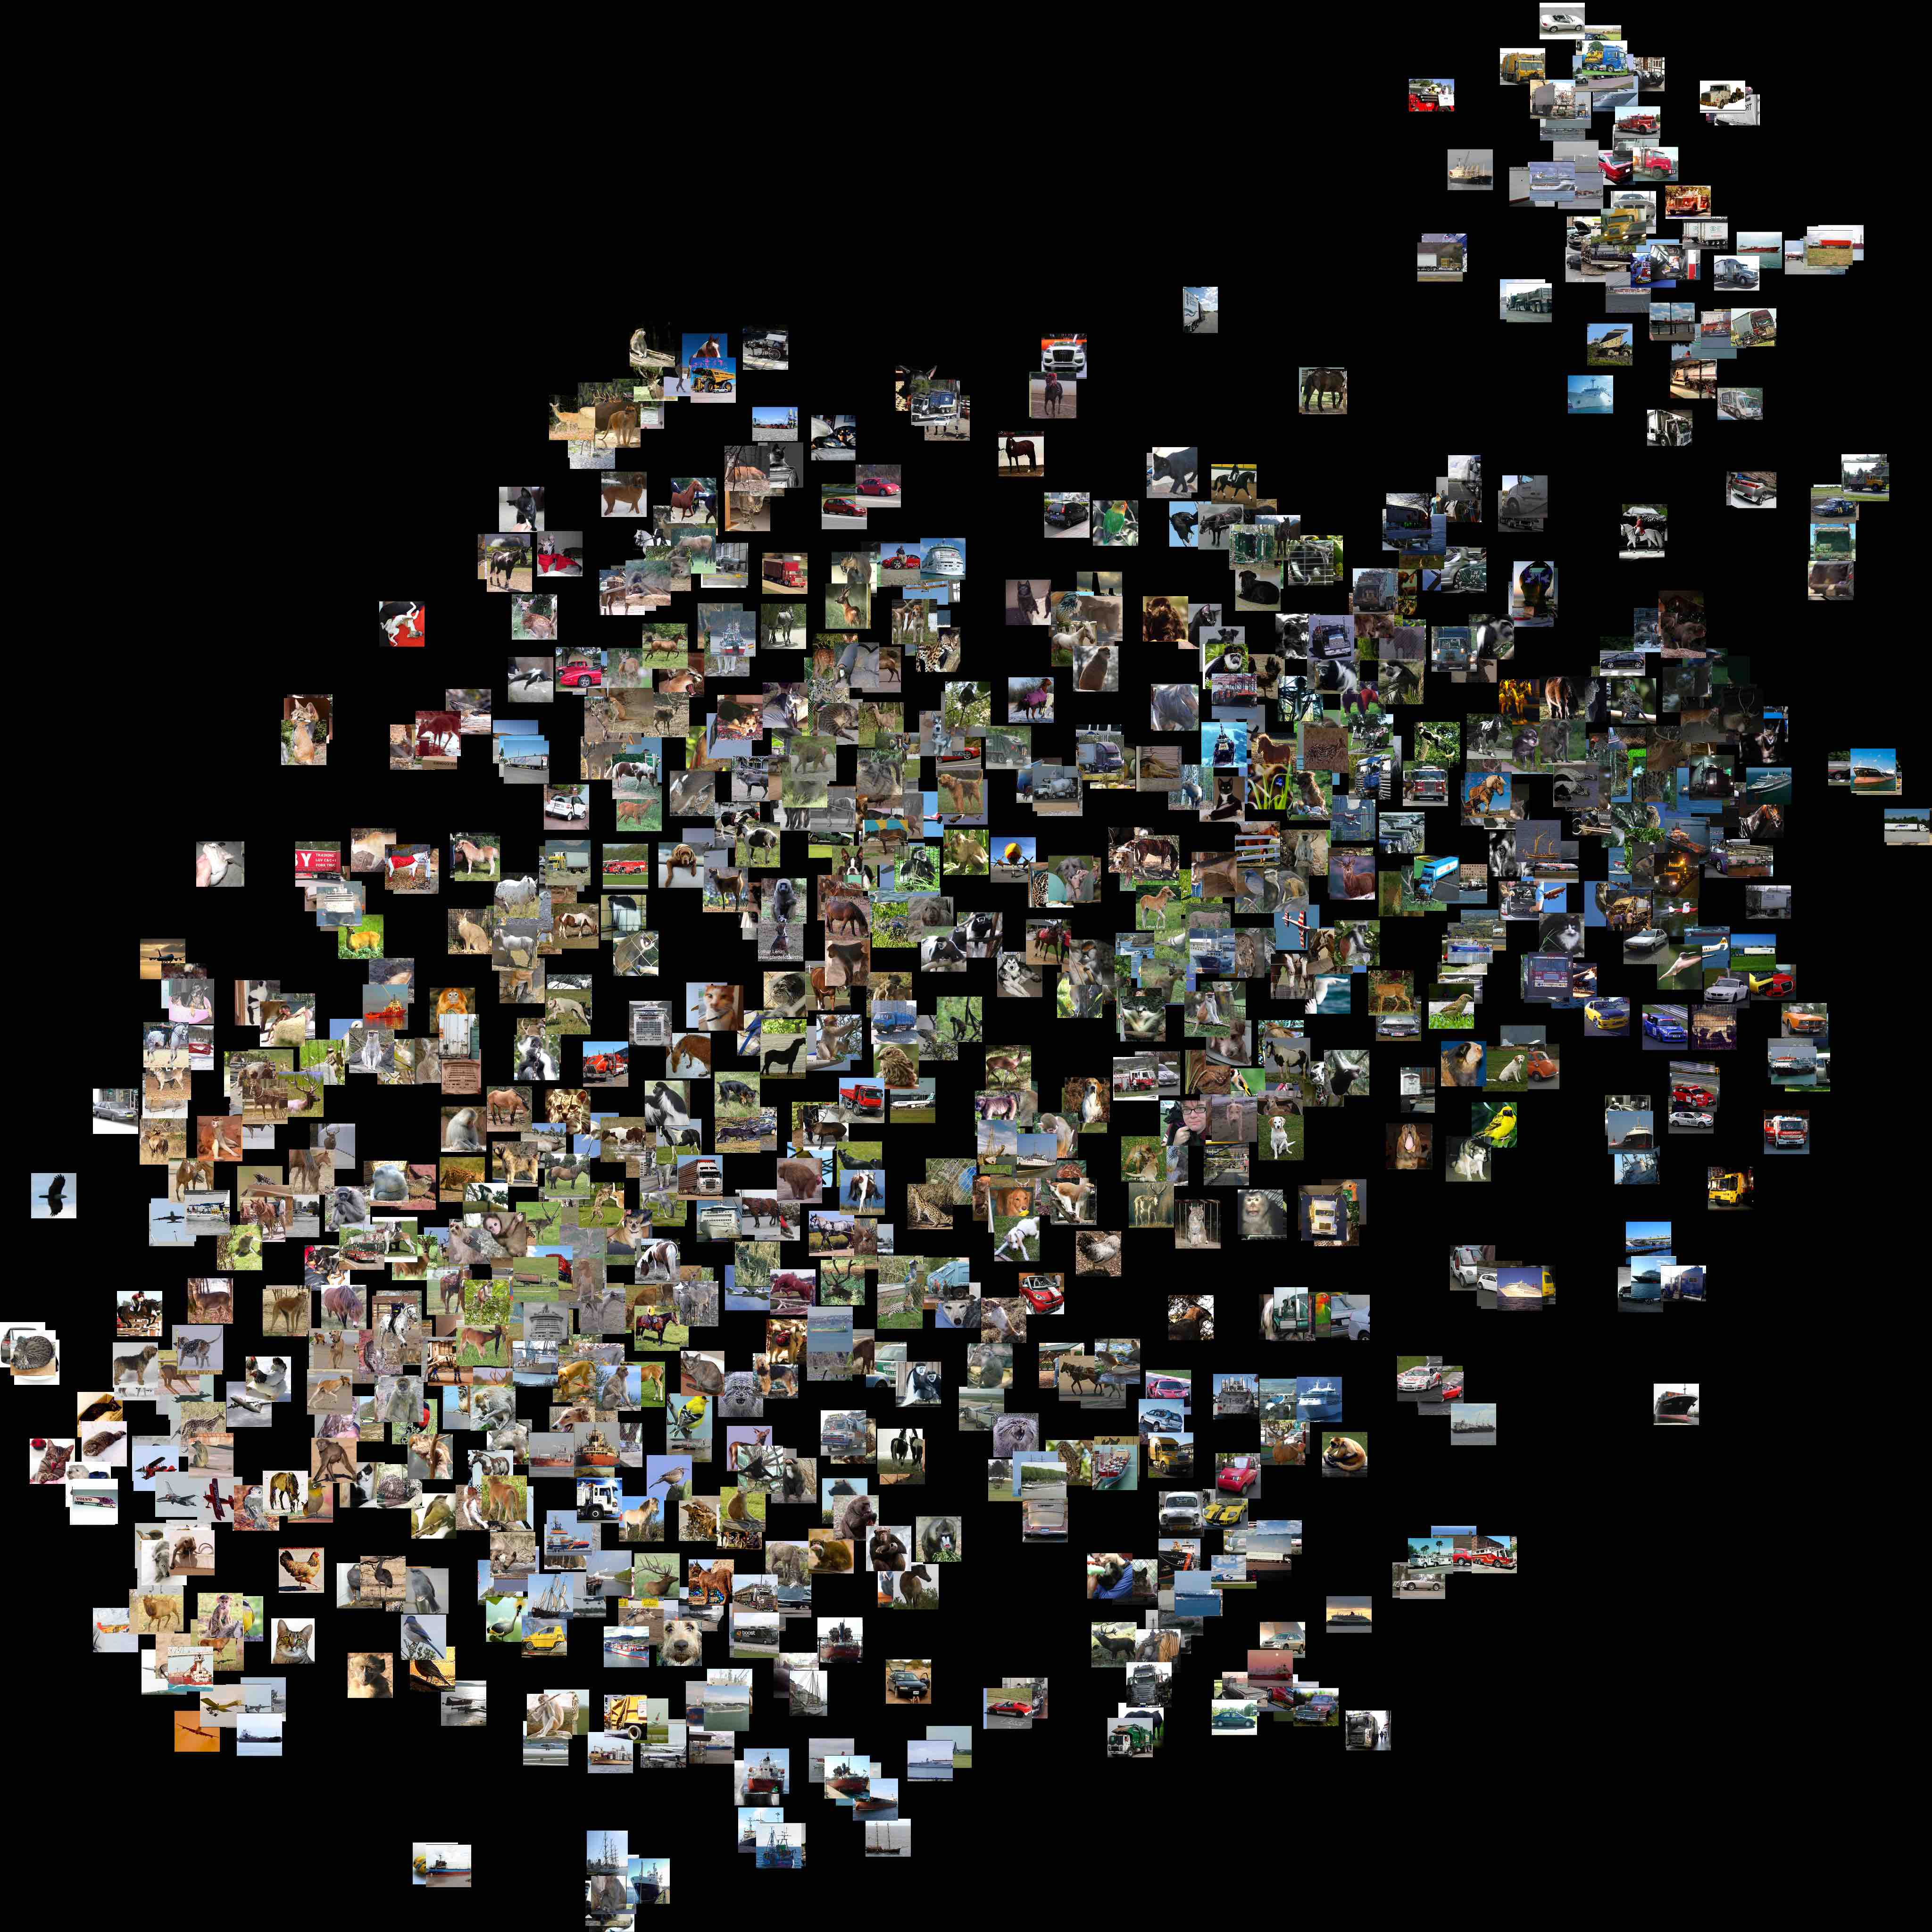
\includegraphics[width=1\textwidth]{../fig/t_SNEIII.jpeg}
  \caption{The training and test accuracy of 3-layer versus 2-layer model}
\end{figure}

\end{document}
